\documentclass[11pt]{article}
\usepackage{geometry}                % See geometry.pdf to learn the layout options. There are lots.
\geometry{letterpaper}                   % ... or a4paper or a5paper or ... 
%\geometry{landscape}                % Activate for for rotated page geometry
%\usepackage[parfill]{parskip}    % Activate to begin paragraphs with an empty line rather than an indent
\usepackage{graphicx}
\usepackage{amssymb}
\usepackage{amsmath}
\usepackage{epstopdf}
\DeclareGraphicsRule{.tif}{png}{.png}{`convert #1 `dirname #1`/`basename #1 .tif`.png}
\setlength{\parskip}{0.5em}

\title{Consumer Price Index Simulation}
%\author{Ted Dunning}
\date{}

\begin{document}
\maketitle
\section{Introduction}
We want to build a fairly realistic simulation of consumer pricing. The basic idea is that we have a basket of goods whose prices roughly follow an overall trend, but with variations imposed by some number of normally unobservable macro-economic effects.

In order to simulate this, we can generate a single scale variable and a number of uncoordinated variables that stand in for macro effects. Each commodity in the basket would have an associated weighting of the macro effects. This weighting can be scaled in order to match a particular initial sample of prices. Pricing of each of the commodities in the basket by combining the scale and weighted macro effects to get a price.

In order to add interest to the simulated prices, we can have either or both of the scale variable and macro effects follow a long-tailed random walk so that we get occasional surprising spikes in the resulting prices.

This model can also handle cases where there are multiple grades of a single commodity such as potatoes by simply including each grade of potato into the sampling basket where the scaling from the macro effects is constrained to be very similar for all of the different grades. Procedurally, this can be done by first picking the macro influence for the combined group and then modifying that base influence slightly for each grade.
\section{Simulating the scale variable and macro-effects}
Desires:
\begin{itemize}
\item Want exponential growth of scale
\item Want long-tailed short-term surprises 
\item Want temporal consistency (i.e. slow change) of macro factors
\end{itemize}
\subsection{Unify scale and macro variables}

Put scale and macro variables into a vector $\mathbf m$. Take the scale variable to be $m_0$ and have it increase by a constant each time step.  Set $m_1=1$ to serve as a bias value for adjusting prices. Index by time so that the value of $\mathbf m$ at time $t$ is written as $\mathbf m[t]$. The $j$-th element of $\mathbf m[t]$ is written as $\mathbf m[t]_j$. The values of this vector are combined in a dot product with each product's parameters to get the log of the final price at a particular time.

Since the final combination of scale and macro factors will be the log of the price, the linear increase in $m_0$ results in exponential increase in prices (neglecting the macro factors).
\subsection{Random walk for macro factors and use $t$-distribution for macro factor steps}
Start with 
\begin{align*}
\mathbf m[0]_0 &= 0 \\
\mathbf m[0]_1 &= 1 \\
\mathbf m[0]_i &= 0 & i > 1
\end{align*}
In this vector $\mathbf m_0$ represents the overall level of inflation and $\mathbf m_1$ is a bias variable that is used to scale the final price for each commodity. Additional values $\mathbf m_i$ where $i>1$ correspond to the macro economic effects. By setting $\mathbf m = e_1$, we make it easy to force the initial price for a particular commodity to any desired value.

To update $\mathbf m$, we add the randomized step $\delta$,
\[
\mathbf m[t+1] = \mathbf m[t] + \delta
\]
where $\delta$ is a random vector variable distributed according to
\begin{align*}
\delta_0 &= \log \alpha \\
\delta_1 &= 0 \\
\delta_i &\sim \sigma t(d) & i > 1
\end{align*}
The number of degrees of freedom $d$ for the $t$ distribution is chosen to provide occasional large jumps. Typically $d \in [1,5]$. The scale factor $\sigma$ is chosen to control how fast the macro factors change. We may want to combine a ``disaster'' macro factor with very small $d$ with other macro factors that are more conventionally behaved and thus have larger values of $d$. The idea of a disaster factor is that it would almost never have a significantly non-zero value (after scaling), but it would occasionally cause a large step resulting in a significant change in prices that depend on that factor. Such a factor could also be constrained to only produce positive steps in pricing.

It may be desirable to add some high-passpass filtering to the macro-economic factors. The purpose of this would be to guarantee that the mean value of the macro factors will be zero, guaranteeing that the average inflation rate is exactly known. Without such filtering, a random walk can wander arbitrarily far from zero. An easy way to implement filtering is to set
\[
\mathbf m[t+1]_i = (1-\mu) \mathbf m[t]_i + \delta
\]
where $\mu_0$ and $\mu_1$ are $0$ and other values are in the range $[0,1)$. For $\mu =0$, we have no filtering effect. For non-zero values of $\mu$, the value of $\mathbf m$ will tend to return to zero as shown in Figure \ref{filtered-random-walk}.
\begin{figure}[htbp]
\begin{center}
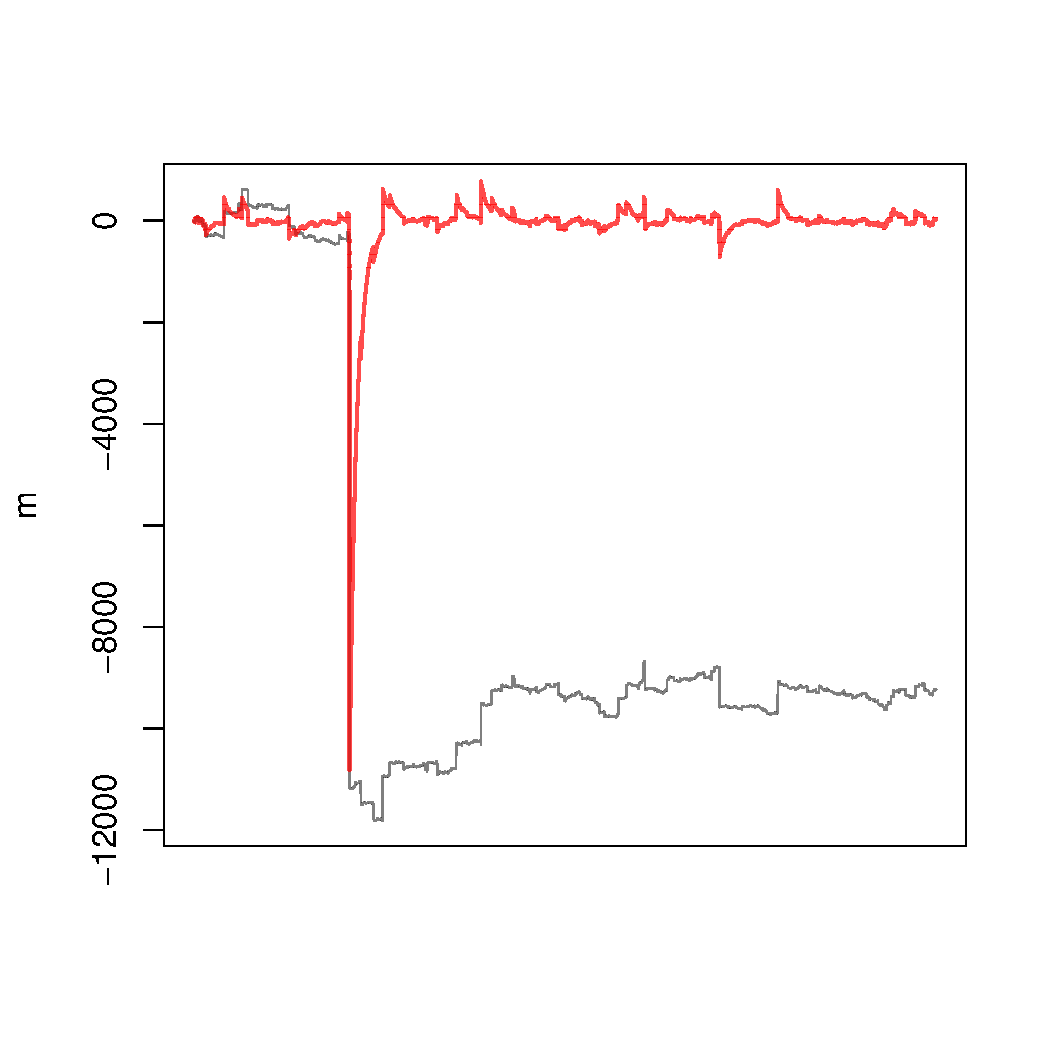
\includegraphics[width=4in, height=3in]{filtered-step.pdf}
\caption{The red line shows what happens when a long-tailed random walk (the black line) is high-pass filtered so that it returns to zero.}
\label{filtered-random-walk}
\end{center}
\end{figure}
The macro factors will have, on average and and after high-pass filtering, zero mean. This means that prices will grow according to $p \approx k e^{\alpha t}$ and the general inflation rate is controlled by $\alpha$ alone. 

\subsection{Treat scale and macros as unified vector for pricing}
The price of a commodity $j$ with influence vector $\mathbf c_j$ can be computed as
\[
\mathbf p_j = \exp (\mathbf c_j \cdot \mathbf m)
\]
The prices of all commodities can be computed in a single step as
\[
 P = \exp ( C \mathbf m)
\]
where the rows of the influence matrix $ C$ are the individual influence vectors for each commodity and the exponentiation is done element by element rather than as a matrix exponential.
\section{Sampling the price influence matrix}
Desires:
\begin{itemize}
\item Want to match original prices at $t=0$
\item Want individual prices to each depend strongly on only a few macro effects
\end{itemize}
By convention, we assume that inflation will affect all prices equally. 
Also note that at $t=0$, only $\mathbf m_1$ will be non-zero. This means that the first two columns of $C$ will consist of two columns that describe the connection to overall inflation and set the price of each commodity at time $t=0$ followed a matrix $H$ that describes the connection between the macro factors and particular prices as in the following structure:
\[
 C = 
\left[
\left.
\begin{matrix}
1&\log p_0  \\
1&\log p_1  \\
\vdots &\vdots &   \\
1&\log p_n & 
\end{matrix}
\right|
H
\right]
\]
Here, $p_j$ represents the price of commodity $j$ at time $t=0$.

The value of $H$ can be sampled at the beginning of each simulation in a number of ways. The simplest would be to simply sample all values from a scaled $t$-distribution. Another option would be to allow different scales and degrees of freedom for each column. A third option would be to use a mixture distribution so that many of the values of $H$ are exactly zero.

\section{Implementation using {\tt {log-synth}}}
%\subsection{}



\end{document}  